%Motivation:
%%%%%%%%%%%%%%%%%%%%%%%%%%%%%%%%%%%%%%%%%%%%%%%%%%
\begin{frame}[fragile]{}

\begin{center}
{
\LARGE
Warum Domain-Driven Design?
}
\end{center}

\end{frame}

%%%%%%%%%%%%%%%%%%%%%%%%%%%%%%%%%%%%%%%%%%%%%%%%%%
\begin{frame}[fragile]{DDD in a Nutshell}

\begin{itemize}
\item Gemeinsames Verständnis schaffen
\item Strukturierung des Codes
\item Trennung Business Logik $\leftrightarrow$ Technik
\end{itemize}

\end{frame}

%%%%%%%%%%%%%%%%%%%%%%%%%%%%%%%%%%%%%%%%%%%%%%%%%%
\begin{frame}[fragile]{Gemeinsames Verständnis schaffen}

\begin{itemize}
\item Hat hohen Stellenwert
\item \glqq Knowledge Crunching\grqq
\end{itemize}

\end{frame}

%Wurde lange Zeit ein bisschen hand-wavey betrachtet: "dann macht man das und dann bekommt man ein gutes Modell"
%%%%%%%%%%%%%%%%%%%%%%%%%%%%%%%%%%%%%%%%%%%%%%%%%%
\begin{frame}[fragile]{}

 \begin{tikzpicture}[remember picture,overlay]
            \node[at=(current page.center)] {
        
\includegraphics[height=\paperheight]{pics/do-knowledge-crunching-and-all-will-be-well.jpg}
            };
\end{tikzpicture}

\end{frame}

%%%%%%%%%%%%%%%%%%%%%%%%%%%%%%%%%%%%%%%%%%%%%%%%%%
\begin{frame}[fragile]{}

 \begin{tikzpicture}[remember picture,overlay]
            \node[at=(current page.center)] {

\includegraphics[height=\paperheight]{pics/one-does-not-simply-do-knowledge-crunching.jpg}
            };
\end{tikzpicture}

\end{frame}

%Dann kam EventStorming auf den Plan
%%%%%%%%%%%%%%%%%%%%%%%%%%%%%%%%%%%%%%%%%%%%%%%%%%
\begin{frame}[fragile]{}

 \begin{tikzpicture}
 % x (kleiner = weiter nach links) y (kleiner = weiter nach unten)
            \put (-10,10) { 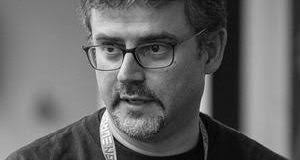
\includegraphics[width=.5\textwidth]{pics/alberto_brandolini.jpg} };
\end{tikzpicture}

\onslide+<2->
 \begin{tikzpicture}
            \put (100,-80) { 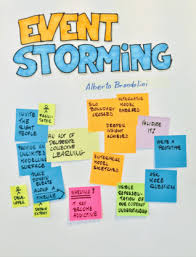
\includegraphics[height=.5\textheight]{pics/eventstorming.jpg} };
\end{tikzpicture}

\onslide+<3->
 \begin{tikzpicture}
            \put (180,-120) { 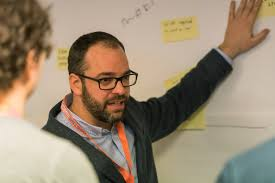
\includegraphics[width=.5\textwidth]{pics/mathias_verraes.jpg} };
\end{tikzpicture}

\end{frame}
% Standing on the shoulders of giants

% Das möchte ich Euch heute vorstellen

%%%%%%%%%%%%%%%%%%%%%%%%%%%%%%%%%%%%%%%%%%%%%%%%%%
\begin{frame}[fragile]{}

\begin{itemize}
\item Wenig Domain-Driven Design
\item Viel gemeinsames Verständnis
\begin{itemize}
\item Knowledge Crunching
\item mit EventStorming
\end{itemize}

\end{itemize}

\end{frame}



%%%%%%%%%%%%%%%%%%%%%%%%%%%%%%%%%%%%%%%%%%%%%%%%%%
\begin{frame}[fragile]{Gemeinsames Verständnis schaffen - Warum?}

\begin{itemize}
\item Gedanken sichtbar und ``begreifbar'' machen
\item Modell schafft Klarheit
\item Ubiquitous Language grenzt Begriffe ab
\end{itemize}

\end{frame}

%Modellieren - warum?
%- Gedanken sichtbar und ``begreifbar'' machen
%- Jeder entwickelt eigene Vorstellung von etwas Gehörtem - Modell schafft Klarheit
%- Dazu gehört Ubiquitous Language - Begriffe sind eindeutig und klar abgegrenzt

% Wenn man etwas hört, macht man sich seine eigene Vorstellung

%%%%%%%%%%%%%%%%%%%%%%%%%%%%%%%%%%%%%%%%%%%%%%%%%%
\begin{frame}[fragile]{}

 \begin{tikzpicture}[remember picture,overlay]
            \node[at=(current page.center)] {
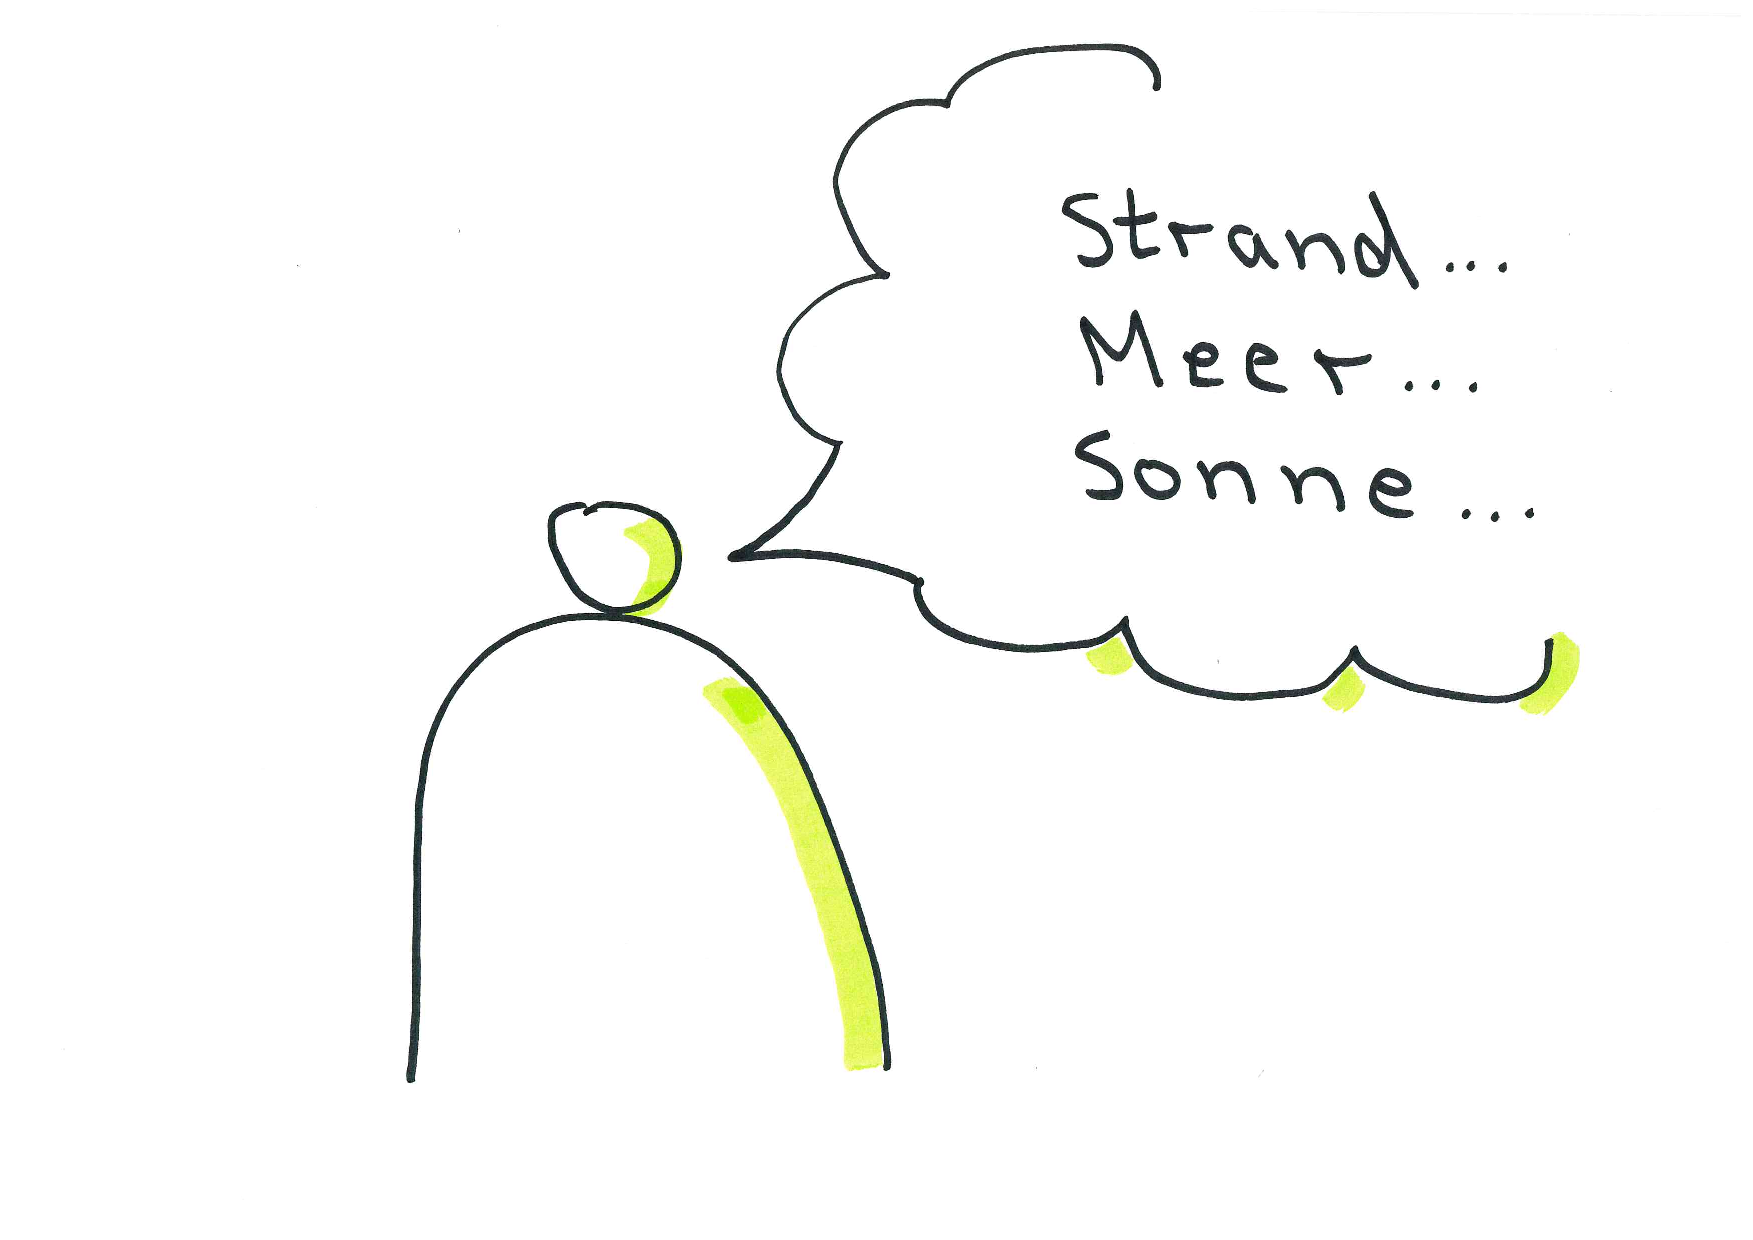
\includegraphics[height=\paperheight]{pics/ich_berichte_von_meinem_urlaub.jpg}
            };
\end{tikzpicture}

\end{frame}

% sonne, strand, meer

%%%%%%%%%%%%%%%%%%%%%%%%%%%%%%%%%%%%%%%%%%%%%%%%%%
\begin{frame}[fragile]{}

 \begin{tikzpicture}[remember picture,overlay]
            \node[at=(current page.center)] {
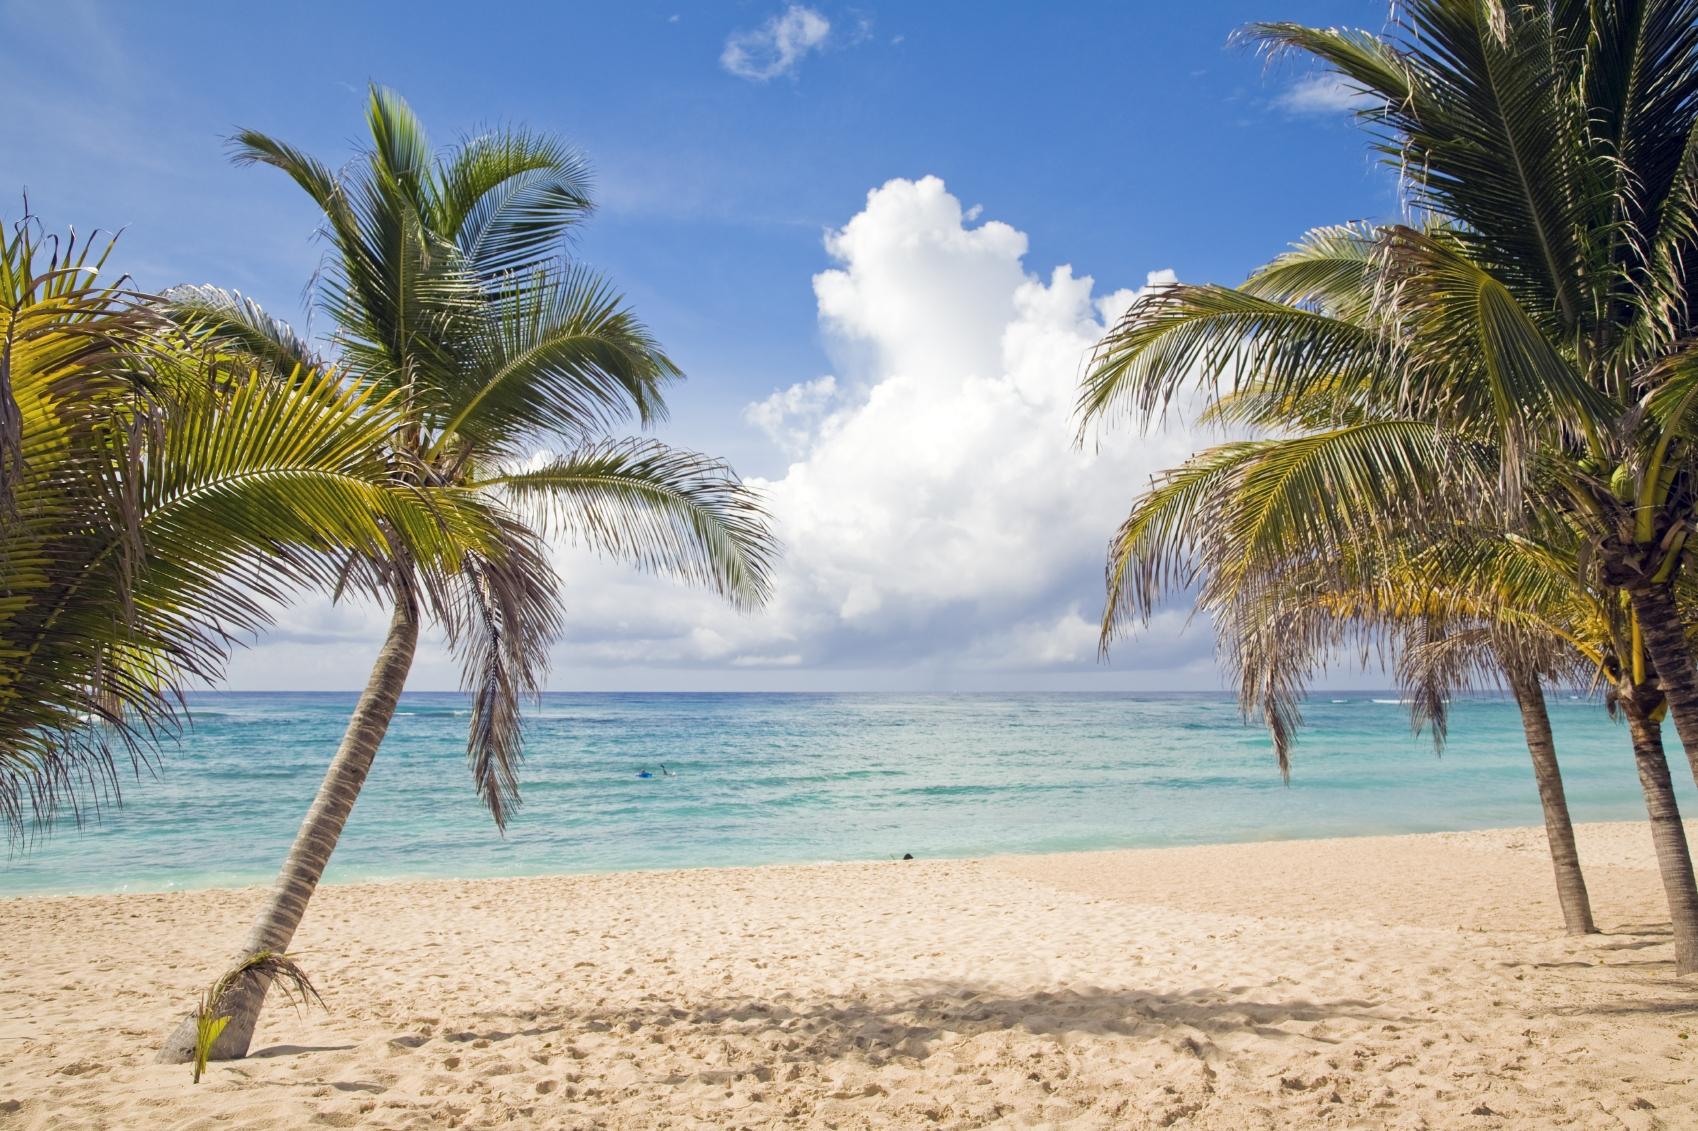
\includegraphics[height=\paperheight]{pics/palm_beach.jpg}
            };
\end{tikzpicture}

\end{frame}

%%%%%%%%%%%%%%%%%%%%%%%%%%%%%%%%%%%%%%%%%%%%%%%%%%
\begin{frame}[fragile]{}

 \begin{tikzpicture}[remember picture,overlay]
            \node[at=(current page.center)] {
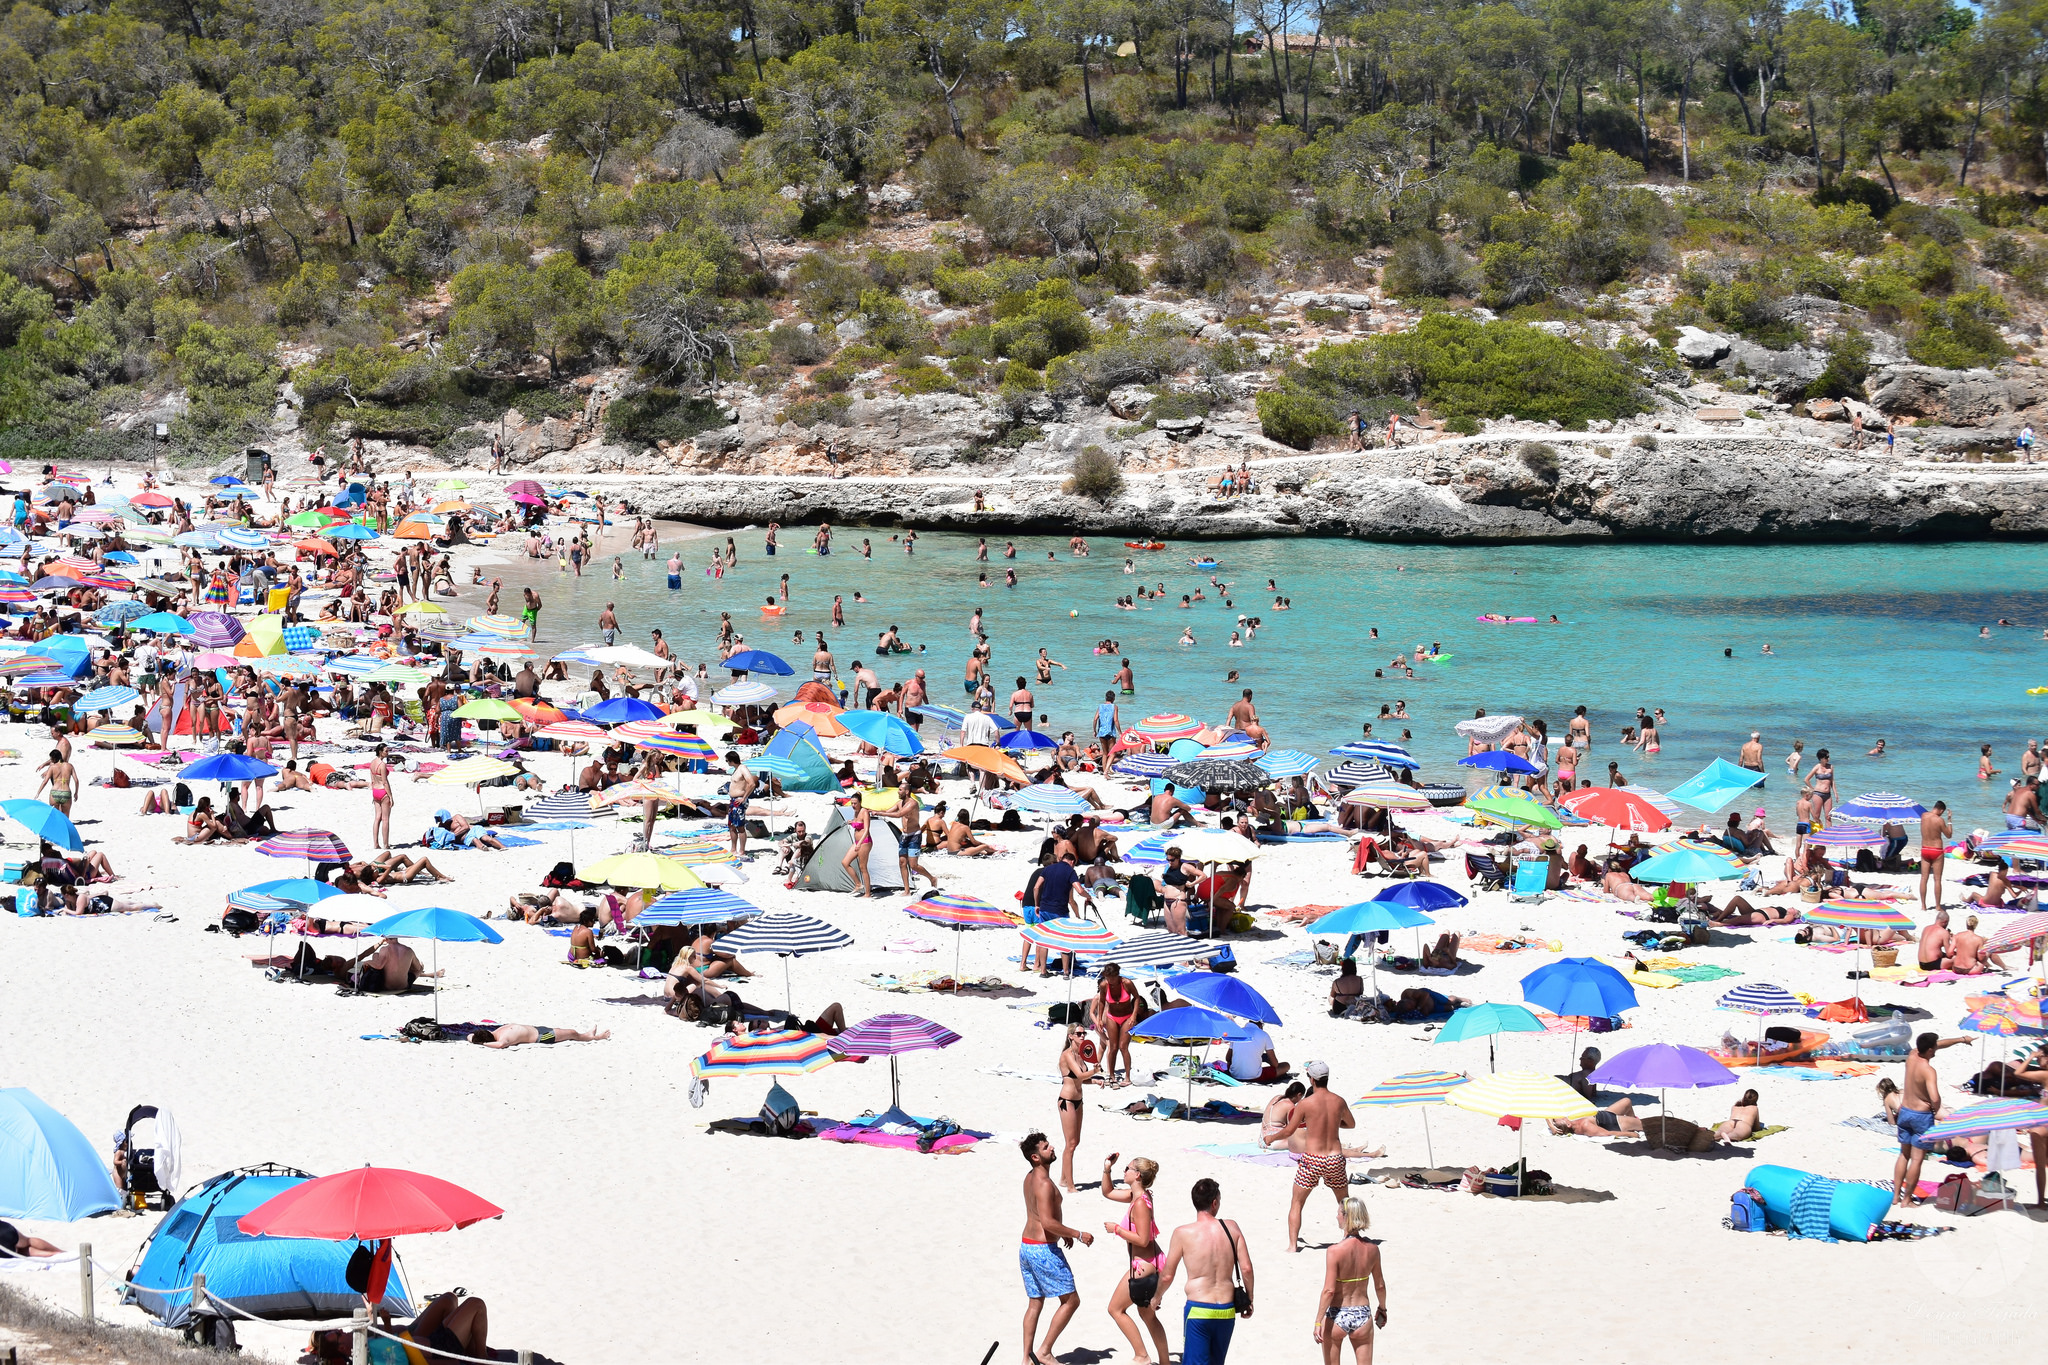
\includegraphics[height=\paperheight]{pics/mallorca_beach.jpg}
            };
\end{tikzpicture}

\end{frame}

%%%%%%%%%%%%%%%%%%%%%%%%%%%%%%%%%%%%%%%%%%%%%%%%%%
\begin{frame}[fragile]{}

 \begin{tikzpicture}[remember picture,overlay]
            \node[at=(current page.center)] {
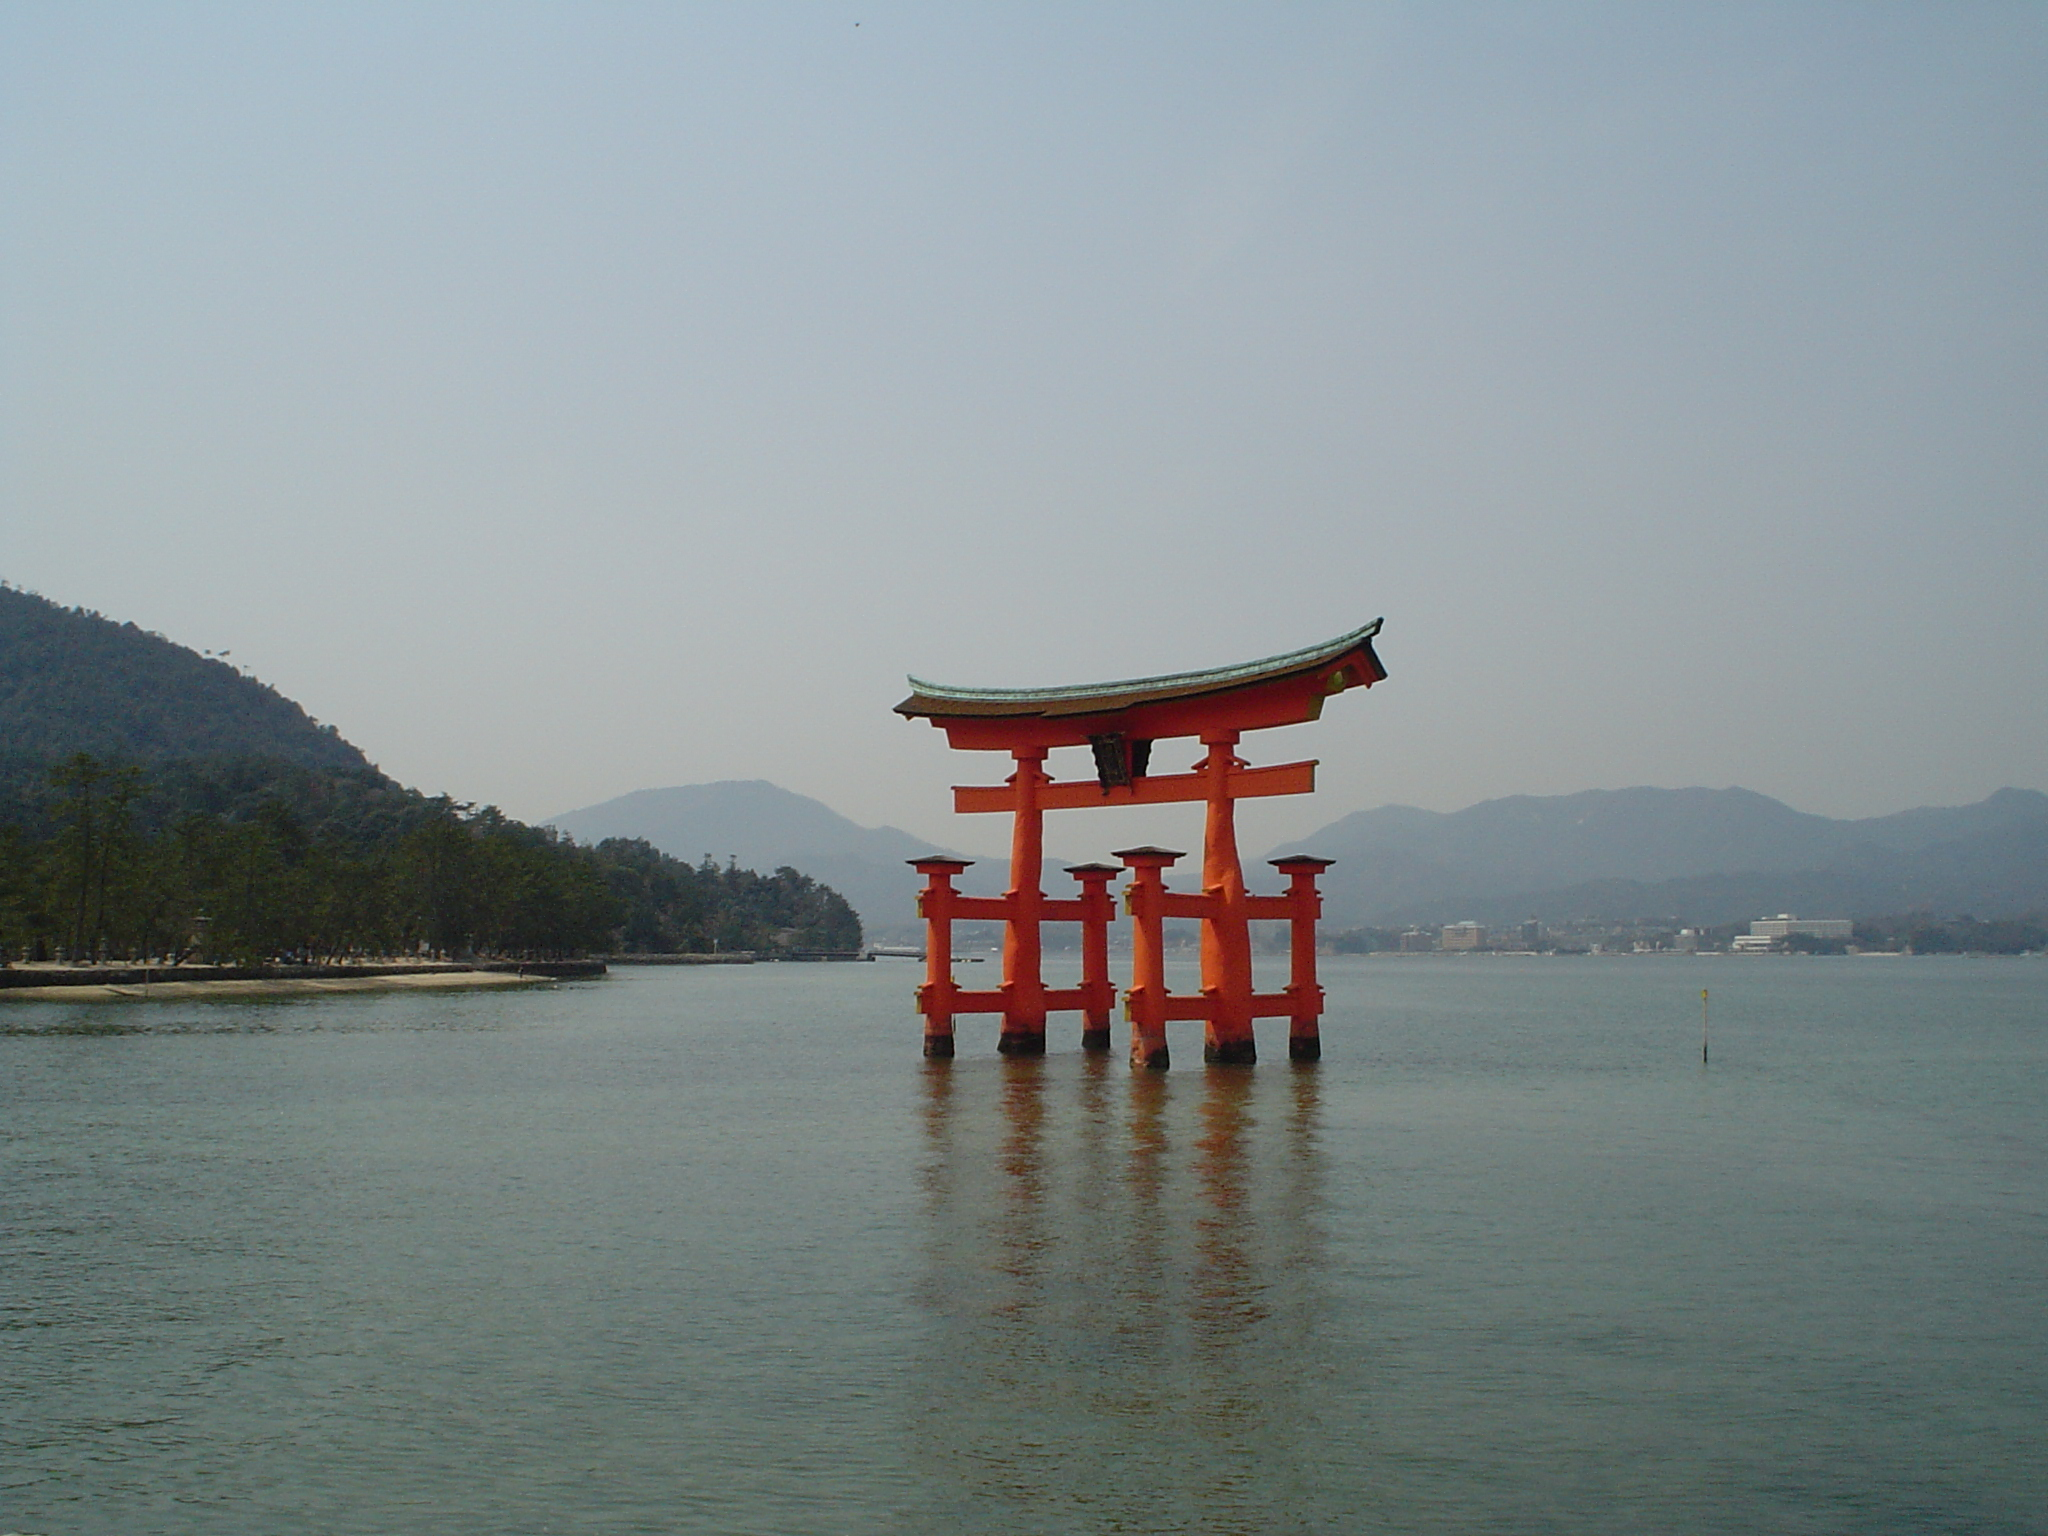
\includegraphics[height=\paperheight]{pics/japan_beach.jpg}
            };
\end{tikzpicture}

\end{frame}

%%%%%%%%%%%%%%%%%%%%%%%%%%%%%%%%%%%%%%%%%%%%%%%%%%
\begin{frame}[fragile]{}

 \begin{tikzpicture}[remember picture,overlay]
            \node[at=(current page.center)] {
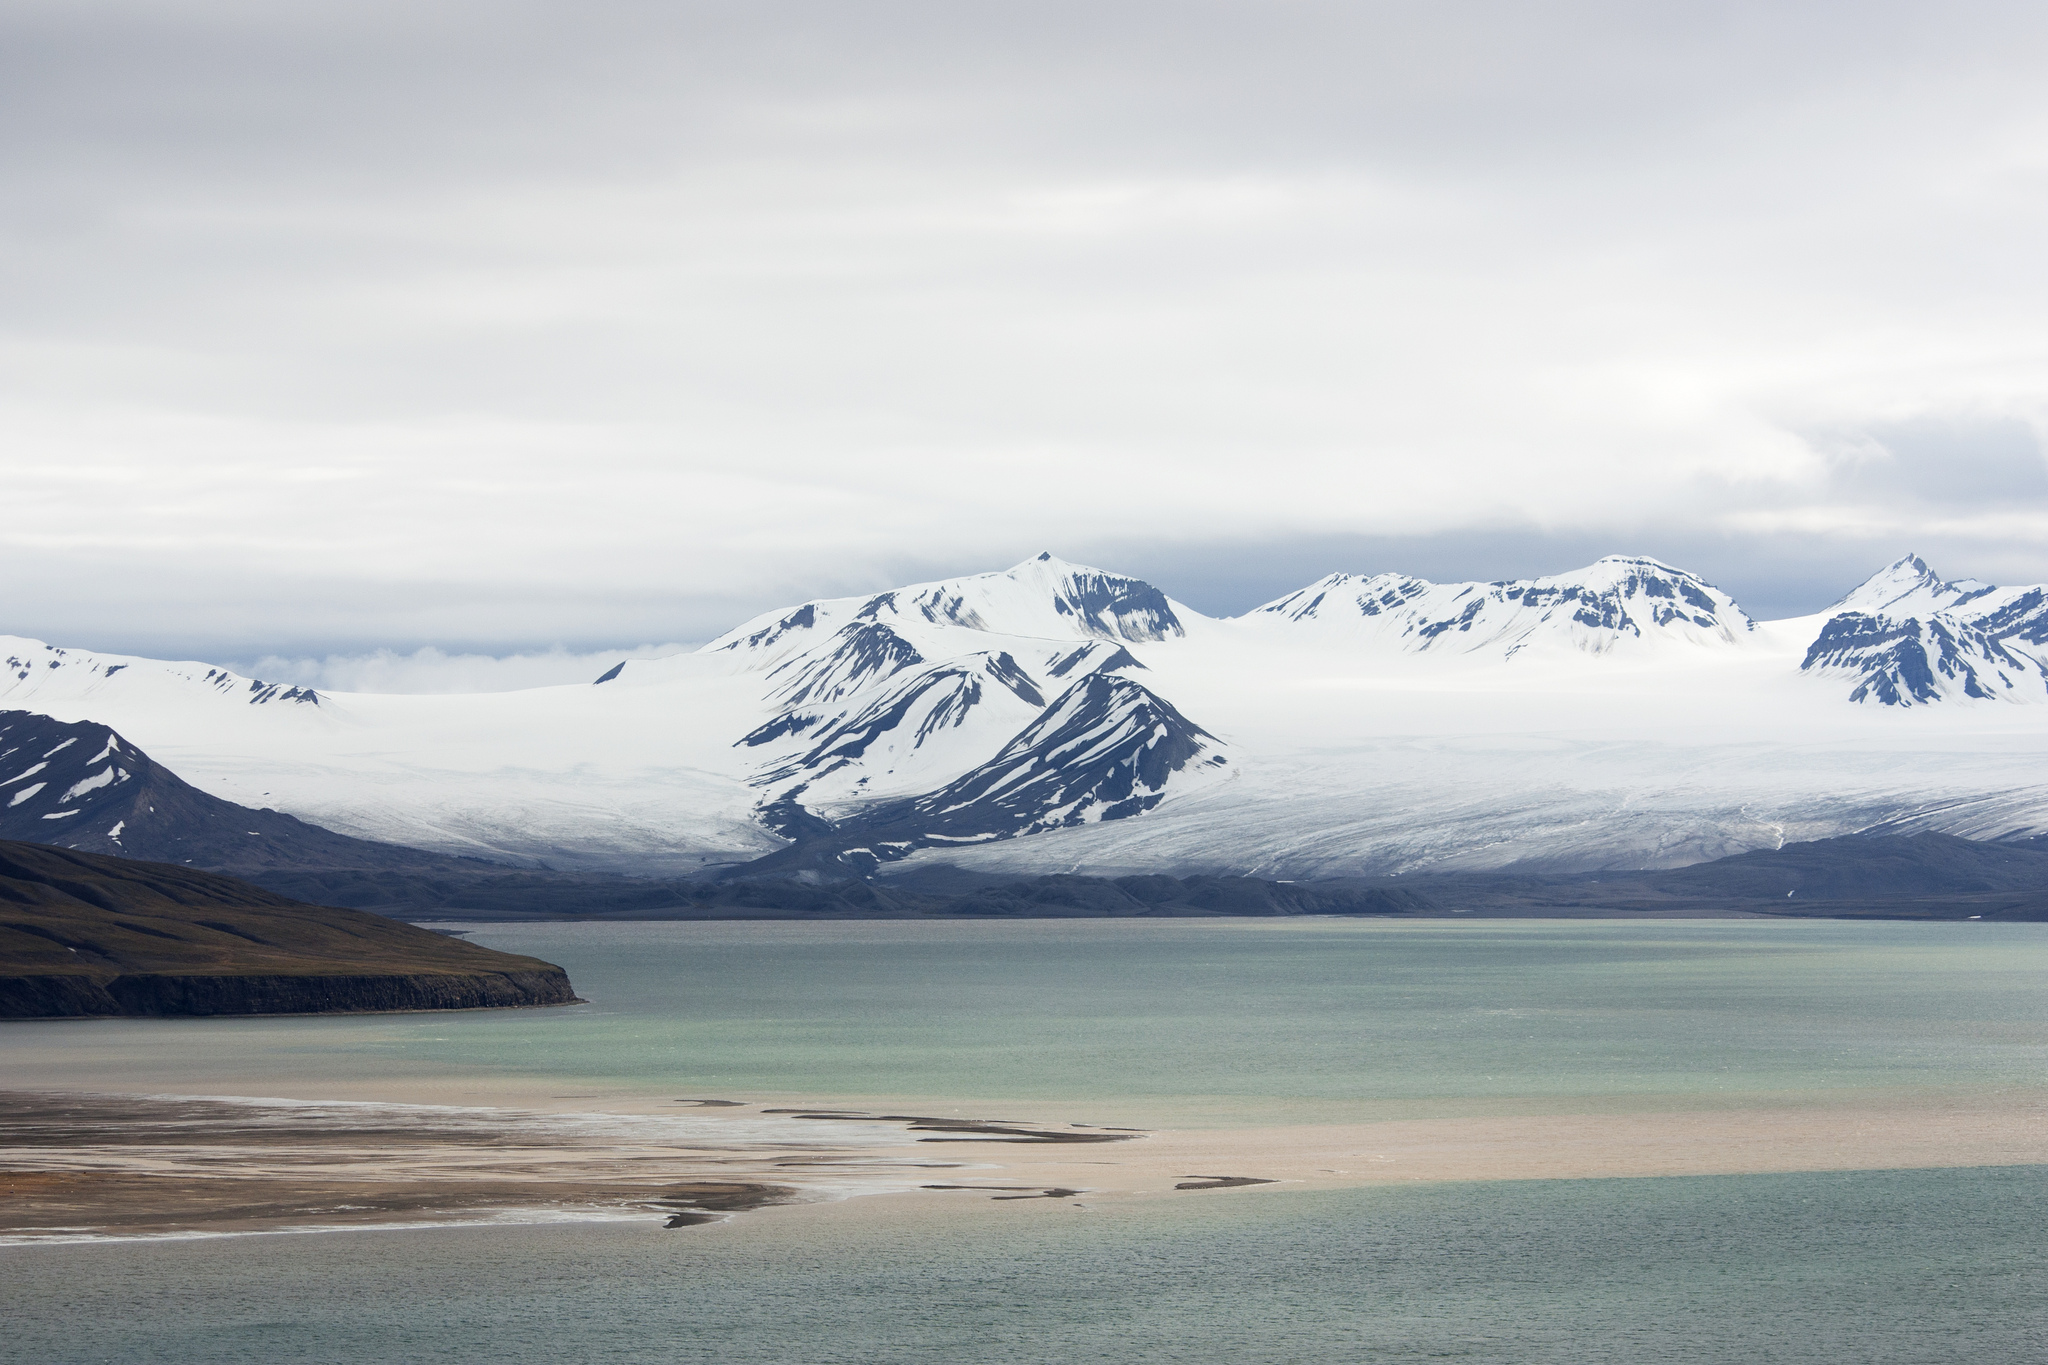
\includegraphics[height=\paperheight]{pics/ice_beach.jpg}
            };
\end{tikzpicture}

\end{frame}

%%%%%%%%%%%%%%%%%%%%%%%%%%%%%%%%%%%%%%%%%%%%%%%%%%
\begin{frame}[fragile]{}

 \begin{tikzpicture}[remember picture,overlay]
            \node[at=(current page.center)] {
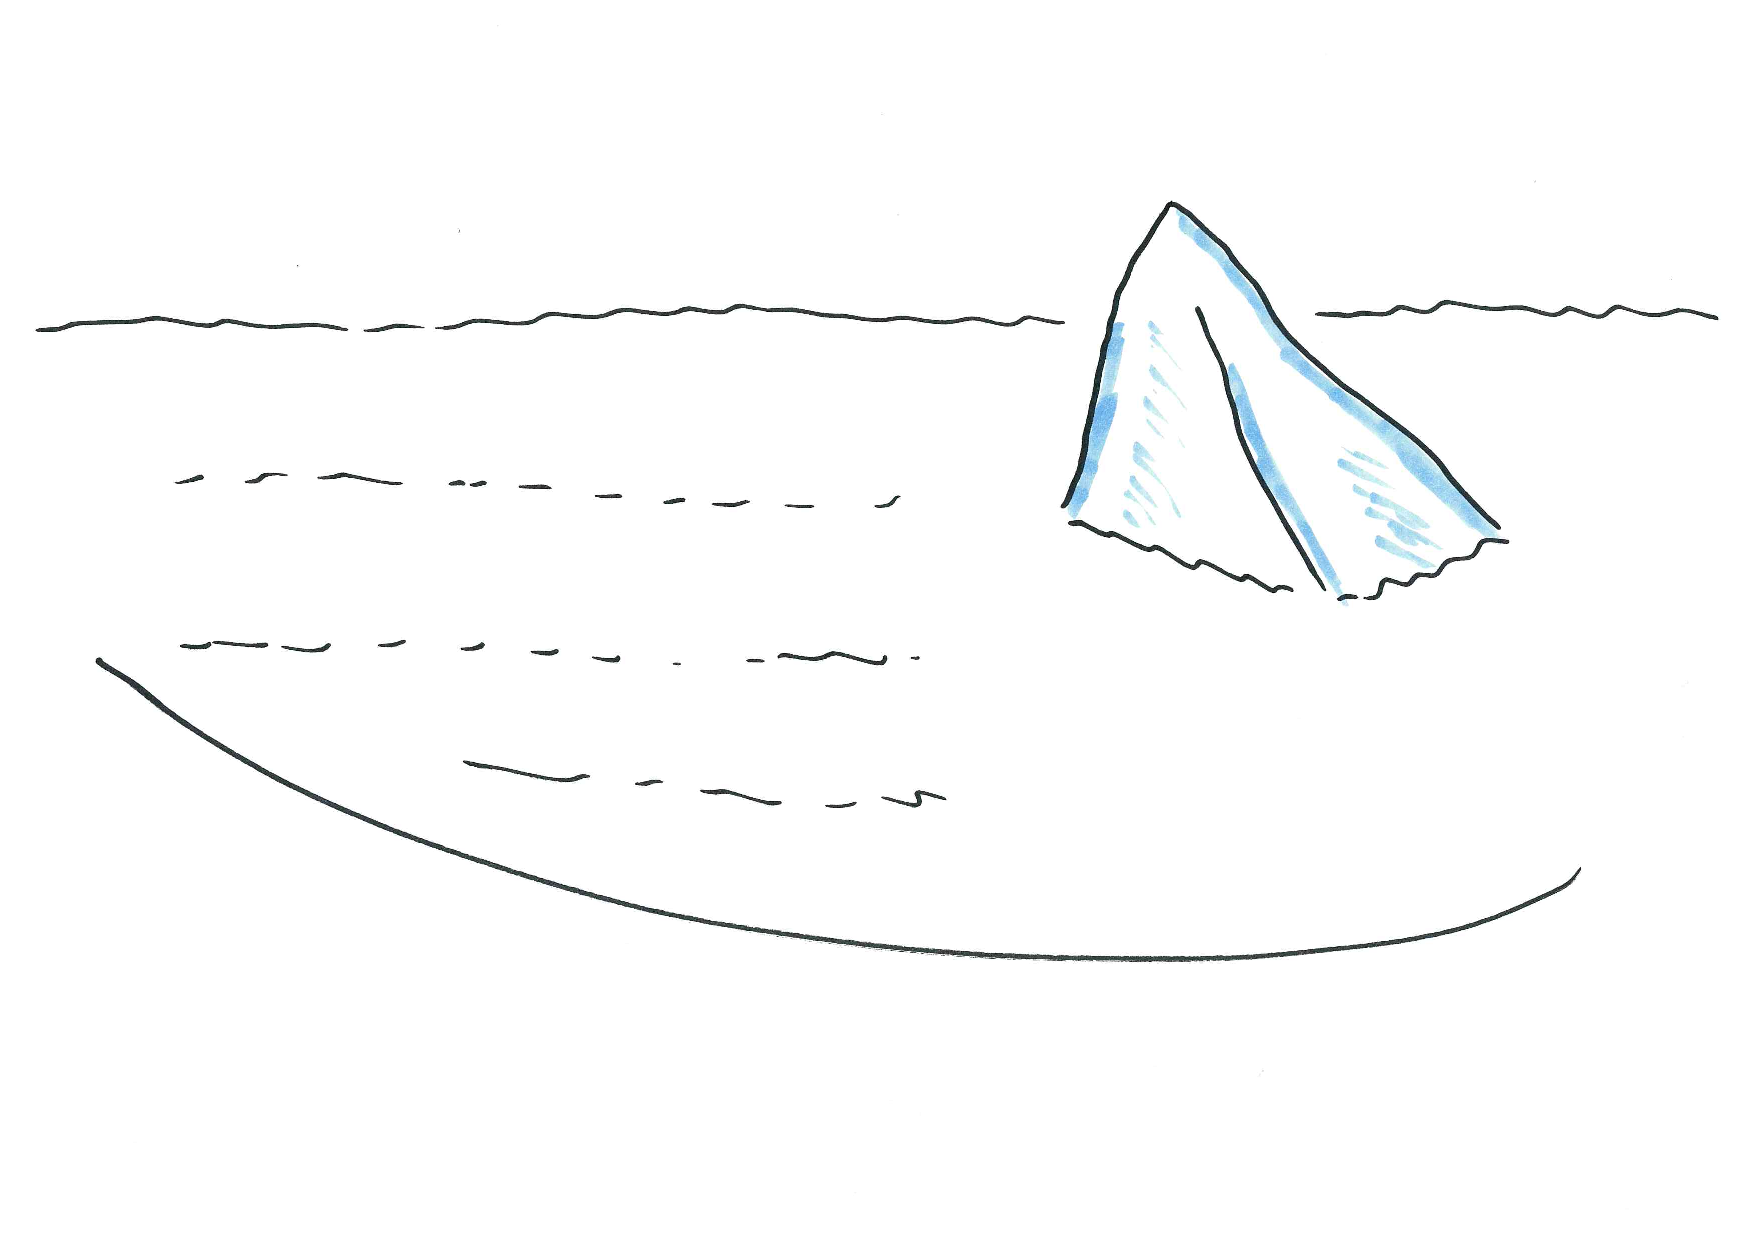
\includegraphics[height=\paperheight]{pics/eine_skizze_meines_urlaubs.jpg}
            };
\end{tikzpicture}

\end{frame}


%%%%%%%%%%%%%%%%%%%%%%%%%%%%%%%%%%%%%%%%%%%%%%%%%%
\begin{frame}[fragile]{WARNUNG}

\begin{center}
{
\LARGE
Hier bei uns passiert gerade dasselbe!
}
\end{center}

\end{frame}

% Vieles, was ich sage, versteht Ihr vermutlich anders als ich es mir vorstelle


%Domäne vorstellen: Orders, Products, Inventory

%%%%%%%%%%%%%%%%%%%%%%%%%%%%%%%%%%%%%%%%%%%%%%%%%%
\begin{frame}[fragile]{Unsere Domäne: eCommerce}

 \begin{tikzpicture}
 % x (kleiner = weiter nach links) y (kleiner = weiter nach unten)
            \put (-10,10) { \includegraphics[width=.5\textwidth]{pics/Produkte.jpg} };
\end{tikzpicture}

\onslide+<2->
 \begin{tikzpicture}
            \put (100,-80) { \includegraphics[height=.5\textheight]{pics/Lagerhaltung.jpg} };
\end{tikzpicture}

\onslide+<3->
 \begin{tikzpicture}
            \put (180,-120) { \includegraphics[width=.5\textwidth]{pics/Bestellungen.jpg} };
\end{tikzpicture}

\end{frame}


Workshop:

1) Events erfassen
Event = Ereignis in der Vergangenheit, das relevant ist für den Fachbereich
Beobachtbar im System


Probleme:
- kein Verb
- nicht in der Vergangenheit
- außerhalb des Beobachtbaren
  - Kunde beginnt sich für unsere Produkte zu interessieren
  - Kunde erhält seine Lieferung


2) Zeitliche Reihenfolge
Redundanzen raus
Fehlendes ergänzen
Ubiquitous Language etablieren

Kritische Fragen:
- Was wenn dies vor jenem passiert?

3) Commands \& Constraints
Commands: Was musste passieren, damit dieses Event stattfinden konnte?
Constraints: Entscheidungen als Frage formulieren, die Events beantworten die Frage
Sauberer modellieren
Clusterbildung
Granularität angleichen
Vollständigkeit checken, Fehlendes ergänzen

Kritische Fragen:
- Folgt dies immer direkt? Gibt es hier keine Constraints?

- Wenn keine Constraints: Entweder Domäne langweilig oder Problem noch nicht verstanden

- Darstellung von Zeit
- Darstellung von Wiederholung

4) Daten zufügen, die bei Entscheidungen und für die Events benötigt werden
Fehlendes ergänzen
Datenquellen identifizieren
Verbindungen schaffen


Debrief

EventStorming auch außerhalb von DDD einsetzbar



Wie geht's weiter?
- Stories schneiden -> Einzel-EventStorming
- Implementieren
- Event Sourced implementieren


%%%%%%%%%%%%%%%%%%%%%%%%%%%%%%%%%%%%%%%%%%%%%%%%%%
\begin{frame}[fragile]{}

\begin{itemize}
\item x
\end{itemize}

\end{frame}

%%%%%%%%%%%%%%%%%%%%%%%%%%%%%%%%%%%%%%%%%%%%%%%%%%
\begin{frame}[fragile]{}

\begin{center}
{
\LARGE
}
\end{center}

\end{frame}

%%%%%%%%%%%%%%%%%%%%%%%%%%%%%%%%%%%%%%%%%%%%%%%%%%
\begin{frame}[fragile]{}

\begin{center}
%\includegraphics[width=\textwidth]{pics/.jpg}
\end{center}

\end{frame}


%%%%%%%%%%%%%%%%%%%%%%%%%%%%%%%%%%%%%%%%%%%%%%%%%%
\begin{frame}{Vielen Dank!}

        Folien: \url{https://github.com/NicoleRauch/FiftyShadesOfParsing} 
        
        ~\\[1em]
        \begin{block}{Nicole Rauch}
        \begin{description}[Twitterxx]
                \item[E-Mail]  \href{mailto:info@nicole-rauch.de}{\texttt{info@nicole-rauch.de}}
                \item[Twitter] \href{http://twitter.com/NicoleRauch}{\texttt{@NicoleRauch}}
                \item[Web] \href{http://www.nicole-rauch.de}{\texttt{http://www.nicole-rauch.de}}
        \end{description}
        \end{block}
\end{frame}

